This layer is responsible for converting the analog signals coming from the layer and receptors subsystem to MIDI signals which can be analyzed by the midi decoder.

\subsection{Layer Hardware}
It consists of Teensy 3.6 micro-controller.

\subsection{Layer Operating System}
Teensy micro-controller is running a arduino script to detect the interference in the laser's circuit.

\subsection{Layer Software Dependencies}
MIDIUSB library is used in order to allow the micro-controller to encode the MIDI signals for the pi.

\subsection{MIDI Encoder}
It is C++ arduino script running on Teensy which converts the analog reading to MIDI signals.

\begin{figure}[h!]
	\centering
 	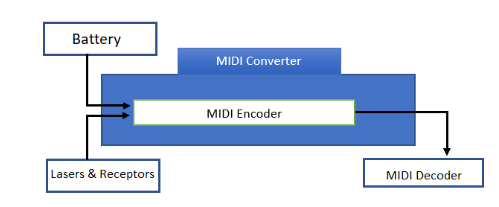
\includegraphics[width=0.60\textwidth]{images/MIDI.png}
 \caption{ MIDI encoder subsystem description diagram}
\end{figure}

\subsubsection{Subsystem Hardware}
Teensy 3.6 180 MHz micro-controller with 32 General purpose DMA channels.

\subsubsection{Subsystem Operating System}
Arduino 1.8 or similar in order correctly run the script.

\subsubsection{Subsystem Software Dependencies}
MIDIUSB library has been used to call functions to send notes or signals to raspberry pi.

\subsubsection{Subsystem Programming Languages}
Basic C++ arduino language is being is used for reading the signals from the circuit.




